\section{Service Oriented Architecture}
\label{fundamentals:service}

In highly dynamic markets, companies must be flexible and adapt their business process quickly to changing environments.
This often includes cooperating or merging with other businesses, business process optimization, or outsourcing.
There have been distributed system technologies in the past that were created to support such dynamic processes on an IT level, but their tight coupling and lack of interoperability resulted in islands of middleware and corresponding application.
The integration between those islands became a new problem that was solved with message oriented middleware~\autocite{webservices}.

Message oriented middleware enables integration of application by wrapping them in adapters.
These adapters are connected with channels which pass along messages.
Channels can ensure a certain quality-of-service, such as exactly-once delivery.
They also can change the messages in other ways, for example by transforming them between different formats.
This allows for loosely coupled communication, since format changes don't affect the ability for two applications to integrate.
The underlying integration middleware can also offer more advanced message exchange patterns, such as asynchronous send and receive or send-and-forget, which further helps with loosely coupled interaction~\autocite{webservices}.

\nom{Service Oriented Architecture}{SOA} is an architecture paradigm that emerged as a result from the lessons learned from the failure of other distributed systems and the success of message-oriented middleware.
It focuses on loose coupling and dynamic binding between services~\autocite{webservices}.
In this case, a service is "a logical representation of a repeatable business activity that has a specified outcome"~\autocite{soa}.
Further characteristics of services are that they are self-contained, that they are composable, i.e. new services can be build by combining multiple other services, and that they are discoverable based on metadata that describes their various aspects.
They also operate like black boxes to their consumers, i.e. no information of how they are implemented or provided is needed to use them~\autocite{webservices}.

\begin{figure}[!htbp]
	\centering
	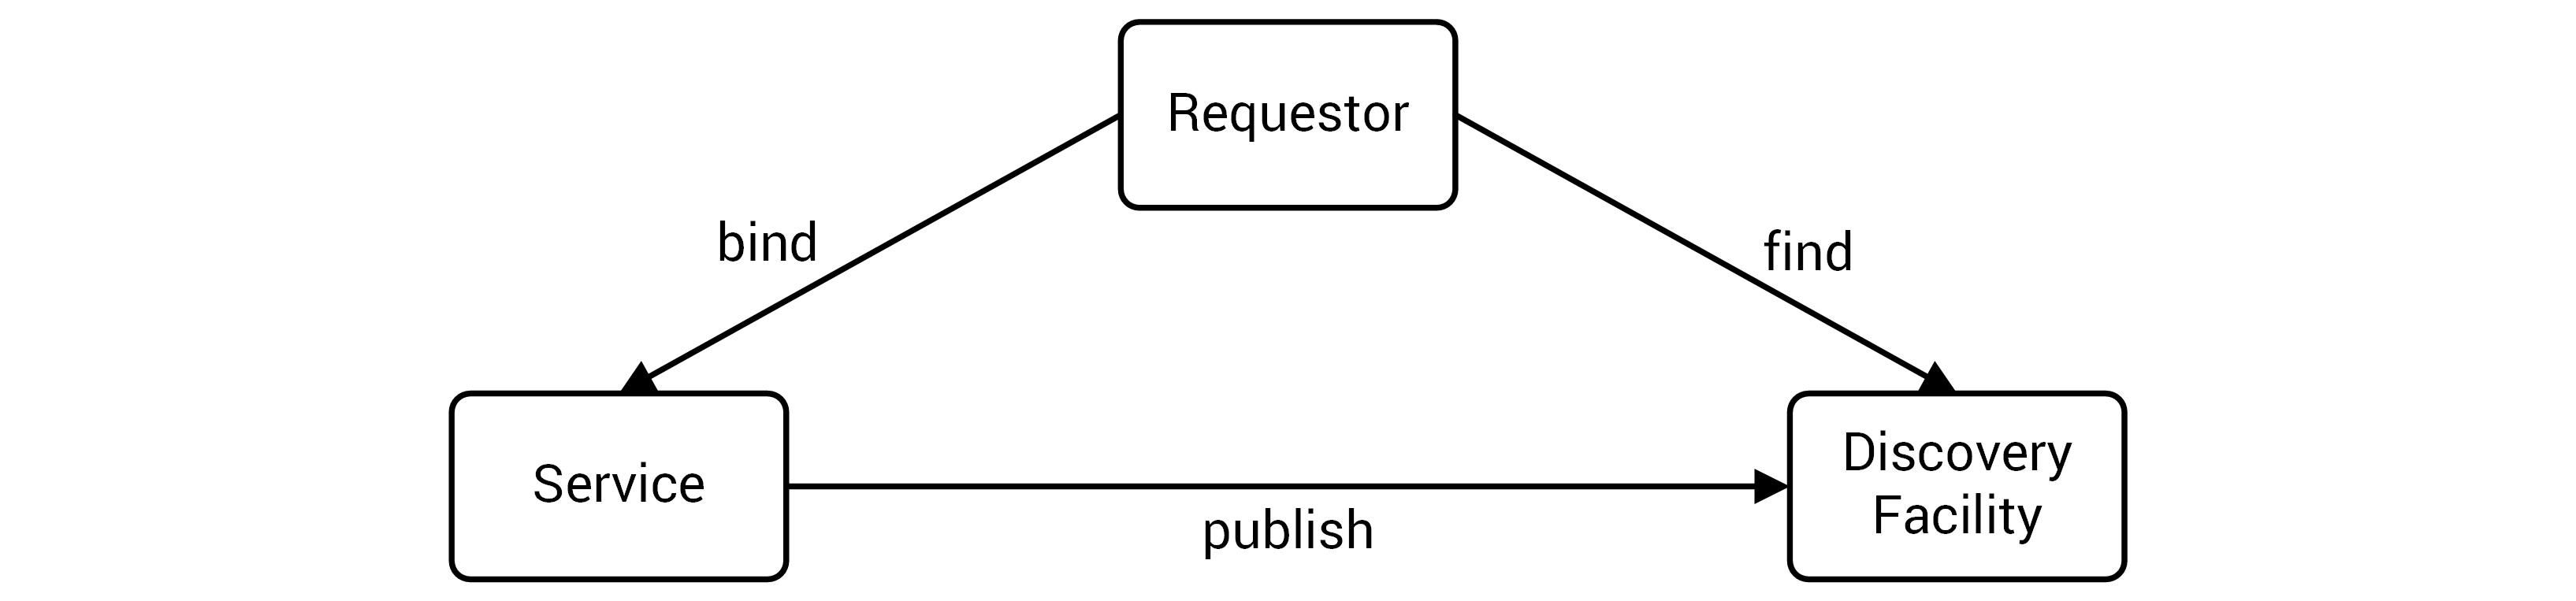
\includegraphics[resolution=600]{fundamentals/assets/triangle}
	\caption{The SOA triangle~\autocite[based on][]{webservices}.}
	\label{image:triangle}
\end{figure}

\autoref{image:triangle} shows the basic principle behind SOA: The SOA triangle, made up of the bind/publish/find approach.
First, a provider creates an abstract definition of a service that includes enough information to allow others to bind to this service.
The provider then publishes metadata describing this service to a directory or registry.
A requestor can then use the discovery facility associated with this registry to find services that fulfills his functional and non-functional requirements, based on the available metadata.
After selecting a service, the requestor then retrieves the corresponding binding information, binds to this service and starts sending requests to it~\autocite{webservices}.

\begin{figure}[!htbp]
	\centering
	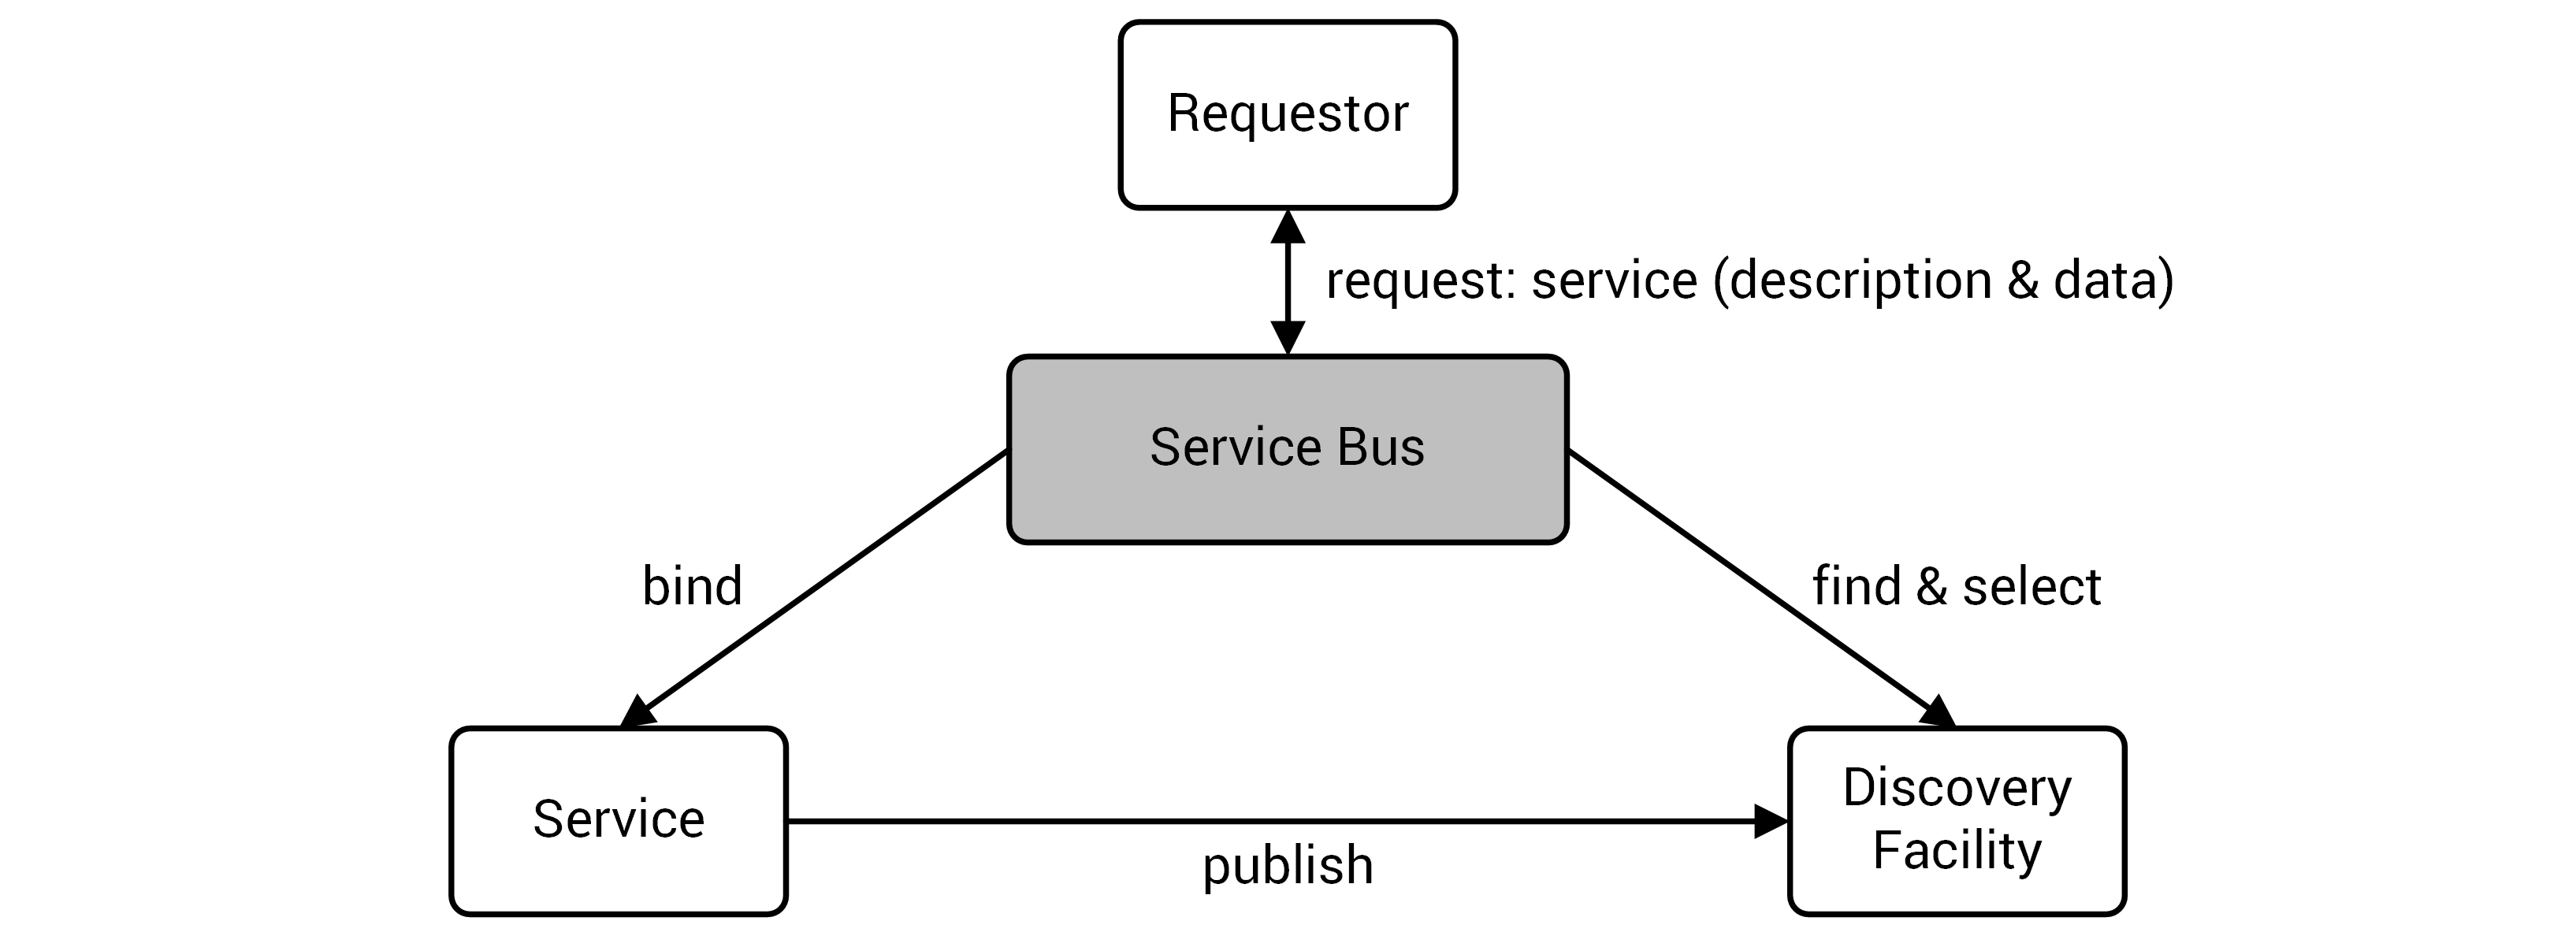
\includegraphics[resolution=600]{fundamentals/assets/service_bus}
	\caption{The SOA triangle including a service bus~\autocite[based on][]{webservices}.}
	\label{image:servicebus}
\end{figure}

To simplify this process for the requestor, a middleware called service bus is introduced, as shown in the middle of \autoref{image:servicebus}.
The requestor now sends the description of the service it intends to use and the data it intends to send to the service to the service bus.
The service bus uses the description to find matching services with the discovery facility, selects one of them, retrieves the binding information and binds to the services.
Then, if necessary, it transforms the data send by the requestor and sends a request to the service.
The response it receives is passed along to the requestor, who now no longer has to deal with any of the above steps~\autocite{webservices}.

Web service technology is one implementation of a service oriented architecture.
It uses wrappers to hide implementation specific functionality and therefor allows applications with different programming models to interact with each other.
To describe these wrappers, the standardized \nom{Web Service Description Language}{WSDL} is used.
WSDL describes the interfaces of the wrappers, which allows a requestor to use any wrapper implementing a particular interface, which creates technology abstraction.
Additionally, quality-of-service descriptions and business-relevant data allow service selection based on business criteria, rather than IT criteria.
This allows requestors to switch dynamically between providers offering identical services with little or no changes to the application, which creates provider abstraction.
\nom{Universal Description, Discovery, and Integration}{UDDI} can be used as a service registry where WSDLs of web services can be published and found~\autocite{webservices}.

A service bus is also at the center of this implementation.
It combines a number of SOA capabilities, specified by numerous web service specifications, to offer the discovery, selection, and binding functionality described earlier.
It can cope with various transport protocols and deal with both XML and non-XML messages.
Quality of service is supported via policies and can include reliable messaging, security, and transaction capabilities.
It also supports atomic services and composed services and provides features for service discovery and negotiation~\autocite{webservices}.
